\subsubsection{Pipeline A}

Since the greenhouse domain provides an highly constrained environment and setup the two main tasks
of canopy segmentation and plant tip location can be solved for very specific cases.

Firstly, it is assumed that only \textit{one} plant canopy per image is visible due to the way the
crop and camera is arranged in the greenhouse - since this is a requirement for the system.

As described in the \ref{subsec:segmentation} this allows a simple segmentation which works well -
as shown in figure \ref{fig:seg:1}, \ref{fig:seg:2}, \ref{fig:seg:3}, \ref{fig:seg:4}.

\begin{figure}[H]
    \centering
    \begin{minipage}[b]{0.24\textwidth}
        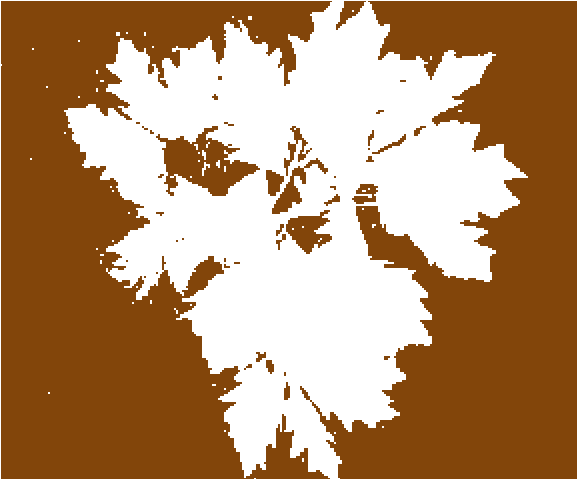
\includegraphics[width=\textwidth]{implementation/segment-1.png}
        \caption{Cluster non-leaf}
        \label{fig:seg:1}
    \end{minipage}
    \hfill
    \begin{minipage}[b]{0.24\textwidth}
        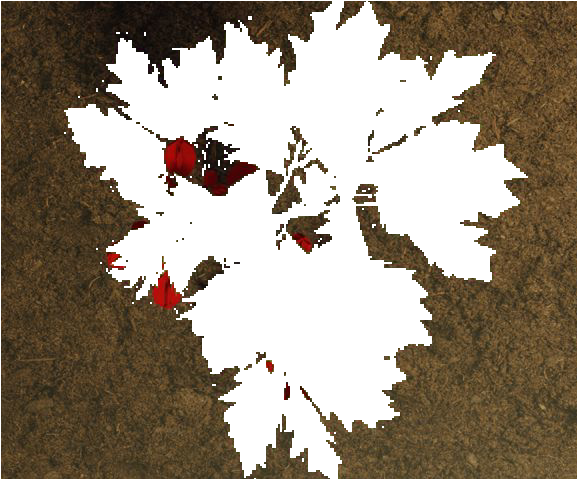
\includegraphics[width=\textwidth]{implementation/segment-2.png}
        \caption{Non-leaf texture}
        \label{fig:seg:2}
    \end{minipage}
    \hfill
    \begin{minipage}[b]{0.24\textwidth}
        \frame{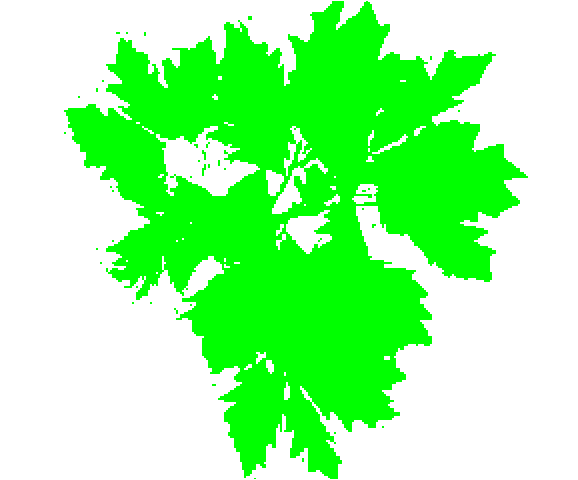
\includegraphics[width=\textwidth]{implementation/segment-3.png}}
        \caption{Cluster leaf}
        \label{fig:seg:3}
    \end{minipage}
    \hfill
    \begin{minipage}[b]{0.24\textwidth}
        \frame{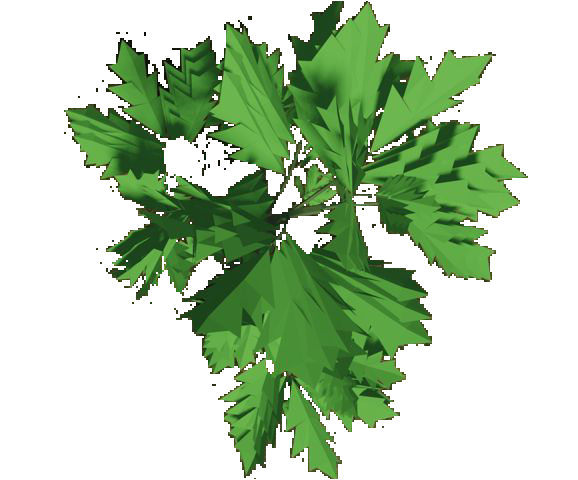
\includegraphics[width=\textwidth]{implementation/segment-4.png}}
        \caption{Texture leaf}
        \label{fig:seg:4}
    \end{minipage}
\end{figure}